\documentclass{article}


% if you need to pass options to natbib, use, e.g.:
%     \PassOptionsToPackage{numbers, compress}{natbib}
% before loading neurips_2021


% ready for submission
\usepackage[preprint]{neurips_2021}
\usepackage[backref=page]{hyperref}
\renewcommand{\backrefxxx}[3]{ p.\hyperlink{page.#1}{#1}}
% \usepackage[hyperpageref]{backref}

\usepackage{graphicx}
\usepackage{caption}
\usepackage{subcaption}
\usepackage[dvipsnames]{xcolor}
\definecolor[named]{ACMBlue}{cmyk}{1,0.1,0,0.1}
\definecolor[named]{ACMYellow}{cmyk}{0,0.16,1,0}
\definecolor[named]{ACMOrange}{cmyk}{0,0.42,1,0.01}
\definecolor[named]{ACMRed}{cmyk}{0,0.90,0.86,0}
\definecolor[named]{ACMLightBlue}{cmyk}{0.49,0.01,0,0}
\definecolor[named]{ACMGreen}{cmyk}{0.20,0,1,0.19}
\definecolor[named]{ACMPurple}{cmyk}{0.55,1,0,0.15}
\definecolor[named]{ACMDarkBlue}{cmyk}{1,0.58,0,0.21}
\hypersetup{colorlinks,
linkcolor=ACMPurple,
citecolor=ACMPurple,
urlcolor=ACMDarkBlue,
filecolor=ACMDarkBlue}
\bibliographystyle{plainnat}
\usepackage[numbers]{natbib}




% to compile a preprint version, e.g., for submission to arXiv, add add the
% [preprint] option:
%     \usepackage[preprint]{neurips_2021}

% to compile a camera-ready version, add the [final] option, e.g.:
%     \usepackage[final]{neurips_2021}

% to avoid loading the natbib package, add option nonatbib:
%    \usepackage[nonatbib]{neurips_2021}

\usepackage[utf8]{inputenc} % allow utf-8 input
\usepackage[T1]{fontenc}    % use 8-bit T1 fonts    % hyperlinks

\usepackage{url}            % simple URL typesetting
\usepackage{booktabs}       % professional-quality tables
\usepackage{amsmath}       % blackboard math symbols
\usepackage{amsfonts}       % blackboard math symbols
\usepackage{nicefrac}       % compact symbols for 1/2, etc.
\usepackage{microtype}      % microtypography
\usepackage{xcolor}         % colors
\usepackage[capitalise]{cleveref}

% \usepackage{subfig}


\usepackage[disable]{todonotes}
\title{\Large Învățare Federată Ierarhică Bidirecțională}

% The \author macro works with any number of authors. There are two commands
% used to separate the names and addresses of multiple authors: \And and \AND.
%
% Using \And between authors leaves it to LaTeX to determine where to break the
% lines. Using \AND forces a line break at that point. So, if LaTeX puts 3 of 4
% authors names on the first line, and the last on the second line, try using
% \AND instead of \And before the third author name.

\author{
  Alexandru-Andrei Iacob \\
  \small Laboratorul de Informatică\\
  \small Universitatea din Cambridge\\
  \small Supervizat de Dr.\ Nicholas Lane\\
  \texttt\small{aai30@cam.ac.uk} \\
  % examples of more authors
  % \And
  % Coauthor \\
  % Affiliation \\
  % Address \\
  % \texttt{email} \\
  % \AND
  % Coauthor \\
  % Affiliation \\
  % Address \\
  % \texttt{email} \\
  % \And
  % Coauthor \\
  % Affiliation \\
  % Address \\
  % \texttt{email} \\
  % \And
  % Coauthor \\
  % Affiliation \\
  % Address \\
  % \texttt{email} \\
}

\begin{document}

\maketitle
% \begin{abstract}
% \input{Files/Abstract}
% \end{abstract}
\section{Introducere}
Învățarea Federată (referită ca FL din termenul englez ``Federated Learning'') este o paradigmă de Învățare Automată Distribuită (referită ca ML din termenul englez ``Machine Learning'')  care permite mai multor clienți să antreneze un model colaborativ comun fără a comunica date private. Aceasta a fost introdusa de \citet{FedAvg} ca un mijloc de reducere a costurilor de comunicare și de diminuare a problemelor de confidențialitate legate de stocarea datelor sensibile într-o locație centralizată. Aceste proprietăți au condus la aplicații FL utilizând grupuri mari de dispozitive de dimensiuni mici, cum ar fi predicția tastaturii mobile~\citep{GoogleKeyboard} pentru telefoanele Android și aplicații cu entități mai mari supuse cerințelor de confidențialitate, cum ar fi spitalele~\citep{FLmedicine}. Aceste două tipuri de Învățare Federată sunt distinse de \citet{AdvancedAndOpenProblems} ca FL cross-device și cross-silo. Pentru restul acestei lucrări un ``client'' se referă la o entitate deținătoare de date private ce efectuează antrenament federat (e.g., telefoane/spitale).

Creșterea preponderenței FL de la publicarea \citet{FedAvg} poate fi atribuită către două trenduri. În primul rând, o creștere a cerințelor de confidențialitate ale consumatorilor și ale cadrului juridic a pus presiune pe companiile de tehnologie. Această presiune a condus la interesul pentru ML care protejează confidențialitatea în cadrul corporațiilor majore precum Google~\citep{FedAvg,GoogleKeyboard,ScaleSystemDesign}, Microsoft~\citep{FLINT} și  Meta~\citep{PAPAYA,FedBuff}. În al doilea rând, ML s-a extins către domenii cu cerințe stricte de confidențialitate precum sănătatea~\citep{FLmedicine}, Recunoașterea Activităților Umane~\citep{HARusingFL_2018,ClusterFL} sau colaborările între corporații~\citep{SustainableIncentive}. Mai mult, apariția Modelelor de Limbaj Mari (referită ca LLM din termenul englez ``Large Language Model'')~\citep{OpportunitiesAndRisksLLM} a făcut accesarea colecțiilor private de limbaj natural avantajoasă, conducând la dezvoltarea FL pentru Procesare a Limbajului Natural~\citep{FedNLP}. În mod similar, lansarea de ponderi~(weights) open pre-antrenate~\citep{LLaMA} permite colaborarea între entități cu resurse computaționale reduse, utilizând framework-uri de FL~\citep{Flower}.

Deși domeniul s-a bucurat de o atenție științifică și industrială sporită, beneficiile pe care le oferă confidențialitatea și comunicarea cauzează provocări semnificative în ceea ce privește creșterea eficienței și evoluția sistemelor federate. În mod crucial, compromisul de a antrena un singur model global nu este potrivit atunci când clienții eterogeni necesită personalizarea parțială sau completă a modelului pentru distribuția lor locală de date.

Această lucrare propune abordarea provocărilor menționate prin construirea de structuri de rețea federate ierarhice de tip arbore, care permit flux de date bidirecțional, unde fiecare frunză este un client, iar fiecare nod intern este un server capabil de antrenament pe date proxy. În consecință, nodurile apropiate de frunze sunt personalizate pentru populația specifică de clienți a subarborelui, iar cele apropiate de rădăcină oferă modele generalizate. Această abordare este denumită Învățare Federată Ierarhică Bidirecțională (referită ca B-HFL din termenul englez ``Bidirectional Hierarchical Federated Learning''). Mai mult, clienții pot executa antrenare asincronă cu modele persistente pentru a aborda shitful în distribuțiile lor de date.
\subsection{Motivație}

În forma sa standard, FL operează direct pe clienți, folosind un server centralizat pentru a distribui parametrii modelului și, apoi, pentru a-i agrega după antrenarea clientului. Acest proces este repetat pentru mai multe runde. Cu toate acestea, datele în FL sunt supuse atributelor precum: locația geografică a clientului, specificațiile senzorului și comportamentul clientului. Datorită acestor factori, distribuția federată încalcă ipoteza Independenței și Identității Distribuției (IID). O astfel de \emph{eterogenitate a datelor}~\citep[sec. 3.1]{AdvancedAndOpenProblems} este împletită cu \emph{eterogenitatea sistemelor}~\citep[sec. 7.2]{AdvancedAndOpenProblems} deoarece clienții au abilități de calcul și viteze diferite de rețea. În plus, costurile de comunicare ale modelului între servere și clienți sunt semnificative. Deoarece eterogenitatea datelor face construirea unui singur model global eficient pentru datele tuturor clienților să fie imposibilă, este propusă crearea unor niveluri arbitrare de personalizare sub forma Învățării Federate Ierarhice într-un mod ce îmbunătățește eficiența și permite evoluția sistemelor.
\subsubsection{Eficiență}

Eficiența și scalabilitatea au fost în centrul cercetării FL de la momentul în care \citet{GoogleKeyboard} a aplicat FL pentru predicția tastaturii mobile de la Google. Pe baza lucrării \citet{GoogleKeyboard}, \citet{ScaleSystemDesign} a demonstrat că FL poate fi folosit pentru a antrena modele în zeci de milioane de smartphone-uri. Cu toate acestea, în ciuda prognozelor optimiste de un miliard de dispozitive ale \citet{ScaleSystemDesign}, au apărut multiple limitări ale eficienței FL. Aceste limitări sunt de trei feluri: (a) FL sincron poate folosi eficient doar sute de dispozitive din miloane în fiecare rundă, (b) antrenarea federată este considerabil mai lentă decât antrenarea centralizată, (c) dispozitivele utilizatorilor sunt nesigure, ceea ce duce la deconectarea acestora. Aceste limitări au primit o atenție suplimentară în evaluarea empirică a \citet{LargeCohorts}.

\citet{LargeCohorts} arată că performanța FL nu se îmbunătățește precum era de așteptat când numărul de clienți antrenați într-o rundă crește, în ciuda lucrărilor teoretice contrare~\citep{TighterTheory}. Rezultatele lor experimentale arată că principala limitare a creșterii dimensiunii grupurilor în setări Non-IID este diferența dintre actualizările de model ale clienților, indicată printr-un cosinus aproape zero între acestea. Această diferență limitează impactul fiecărei runde, provoacă randamente diminuate la creșterea dimensiunii grupurilor și rezultă în incapacitatea de a învăța eficient din datele clienților. Astfel, având în vedere că algoritmii FL sunt intrinsec paraleli, scalabilitatea lor este limitată de capacitatea de a învăța eficient pe baza fiecărui exemplu de antrenament al clienților. În plus, în timp ce investigațiile originale ale \citet{ScaleSystemDesign,LargeCohorts} erau cross-device, problema învățării eficiente de la clienți se aplică și situațiilor cross-silo.


\subsubsection{Evoluție}
Seturile de date ale clienților care formează o rețea federată nu sunt în general statice. Clienții pot șterge datele imediat după generare, periodic sau ad-hoc, în funcție de necesitățile de memorie sau de cererile proprietarului. În plus, caracteristicile datelor nou adăugate se pot modifica în timp într-un mod gradat sau imediat. De exemplu, în sarcinile de recunoaștere a imaginilor, tranzițiile sezoniere pot modifica încet imaginile capturate, în timp ce schimbarea locațiilor sau actualizarea hardware-ului camerei poate duce la schimbări discrete. Această problemă este cunoscută sub numele de ``shift'' al setului de date~\citep[sec. 3.1]{AdvancedAndOpenProblems} și reprezintă eterogenitatea \emph{în-client} mai degrabă decât eterogenitatea \emph{între-clienți}, mai comună. Algoritmii sincroni de Învățare Federată~\citep{FedAvg,FedOPT,QFedAvg} presupun că antrenarea clienților se realizează doar pe modelul federat primit la începutul unei runde. Chiar și sistemele ce mențin modele locale persistente~\citep{Ditto}, presupun că acest model persistent este folosit doar în timpul rundelor FL. Prin urmare, abordările actuale nu pot capta schimbările în distribuția datelor unui client. Sistemele asincrone de FL~\citep{AsynchronousFLonHetDevicesSurvey,FedBuff}, precum PAPAYA de la Meta~\citep{PAPAYA}, permit clienților să fie utilizați în afara limitelor unei runde. Cu toate acestea, ele consideră antrenarea clienților doar pe cea mai recentă versiune accesibila a modelului federat.

\subsection{Rezumatul propunerii}

Această propunere extinde lucrările realizate de \citet{EuroMLSysWorkshop} și \citet{OperaWorkshop} pe subiectele de Învățare Federată personalizată, respectiv ierarhică. Sistemul propus comunică datele într-o structură de tip arbore, așa cum este ilustrat în \cref{fig:TreeStructure}. În mod crucial, parametrii modelelor pot circula în ambele sensuri, iar nodurile pot aplica actualizări parțiale de la părinții lor prin agregare. În plus, fiecare nod poate asocia o pondere diferită parametrilor copiilor și părinților în timp ce folosește metode precum optimizatori adaptivi de server~\citep{FedOPT} sau cele bazate pe antrenare~\citep{Ditto,EWC,DeepMutualLearning}. Algoritmii adaptivi sunt relevanți deoarece permit fiecărui nod din arbore să se distingă în funcție de starea sa anterioară, fără a necesita ajustarea suplimentară a parametrilor. În final, în cazul în care grupurile de clienți sunt construite în mod semantic, această structură poate permite o creștere drastică a eficienței sistemului, deoarece fiecare cluster decide cum să optimizeze între generalizare și personalizare~\citep{PersonalisationGeneralisationTradeoff}. Contribuțiile potențiale ale propunerii includ:
\begin{enumerate}
    \item O familie de algoritmi FL ierarhici și scalabili care permit un control fin asupra personalizării și generalizării de la rădăcina globală până la frunzele complet personalizate.
    \item Investigarea a trei tehnici complementare permise de aceste structuri ierarhice: (a) permiterea frunzelor (clienților) să mențină modele locale persistente care se antrenează asincron pentru a aborda shiftul temporal al setului de date, (b) capabilitatea ca orice nod din arbore să se antreneze cu un set de date proxy pentru a injecta o perspectivă generală modelului, (c) construirea de conexiuni verticale suplimentare în arbore similare cu conexiunile reziduale~\citep{ResNet} pentru a permite un flux de date modificabil fără a schimba infrastructura de comunicare.
    \item Evaluări empirice extinse care iau în considerare scenarii cu sau fără clustere semnificative de clienți în sarcini de recunoaștere a limbajului sau, dacă timpul permite, a vorbirii umane.
    \item O lucrare științifică care este menită publicării la conferința \href{https://iclr.cc/}{ICLR} sau \href{https://mlsys.org/}{MLSys}. Această publicație va fi urmată de o lucrare destinată pentru conferința \href{https://sigmobile.org/mobicom/2023/}{MobiCom} ce investighează antrenamentul asincron pe dispozitive cu resurse limitate, cu shift de set de date, folosind clusterul Raspberry Pi FL din laboratorul Cambridge ML Systems.
\end{enumerate}

\section{Publicații anterioare}
Propunerea din acest document a apărut drept consecință naturală a cercetărilor privind Învățarea Federată Personalizată și Învățarea Federată Ierarhică efectuate în timpul Masterului meu în Informatică Avansată și în primul an al doctoratului meu în laboratorul Cambridge ML Systems, condus de Dr. Nicholas Lane.

\citet{EuroMLSysWorkshop} a investigat compromisul dintre generalizare și personalizare, care este în centrul acestui studiu, din perspectiva ``Fair'' FL~(FFL) și a interacțiunilor sale cu adaptarea locală~(fine-tuning) a modelului federat post-antrenament. Deoarece FFL încearcă să construiască o distribuție mai uniformă a acurateții pentru modelul federat pe seturile de date de testare locale ale clienților, așteptarea era fie reducerea necesității personalizării, fie oferirea unui punct de plecare mai avantajos din care să fie efectuată adaptarea locală. Rezultatele experimentale au arătat că FFL nu aduce beneficii. În schimb, are potențiale dezavantaje pentru aplicarea ulterioară a adaptării. Aceste dezavantaje au dus la propunerea unui algoritm FL conștient de personalizarea ulterioară (``Personalisation-aware Federated Learning'') care încearcă să anticipeze funcțiile de cost comune, utilizate în timpul fine-tuning-ului pe parcursul procesului FL.

\citet{OperaWorkshop} a evaluat performanța Recunoașterii Activităților Umane Federate~\citep{HARusingFL_2018} folosind date multimodale adunate de la diferite tipuri de senzori. Scopul era evaluarea efectului menținerii datelor în cadrul stocării private, cu un nivel crescător de confidențialitate. Studiul a demonstrat că gruparea clienților în funcție de tipul de senzor care a produs setul lor de antrenament atenuează eficient impactul necesității de confidențialitate la nivel de subiect uman, de mediu și de senzor. Această lucrare a fost un precursor direct al B-HFL, deoarece se baza pe o structură de model în două niveluri în care fiecare client antrenează atât un model la nivel de grup, cât și modelul federat global, folosind o abordare de învățare mutuală~\citep{DeepMutualLearning}. Această lucrare a fost ulterior extinsă pentru a lua în considerare adaptabilitatea unor astfel de sisteme la adăugarea unui nou tip de senzor~(grup) în federație; extinderea a fost trimisă simpozionului \href{https://mobiuk.org/2023}{MobiUK}. Învățarea mutuală a fost aleasă pentru a relaționa modelele la nivel de grup cu cel global, deoarece permite utilizarea de arhitecturi divergente ce împart doar stratul final. In ciuda succesului său, această metodă de antrenament necesită ca potențialii clienți să aibă o cantitate mare de date și resurse pentru a antrena modele. Natura costisitoare a procedurii a impus o mișcare spre o abordare bazată pe agregarea modelelor.

Ambele lucrări anterioare au fost implementate în cadrul framework-ului Flower~\citep{Flower}. Cu toate acestea, scara experimentării necesare pentru validarea completă a B-HFL ar fi nerealizabilă pe motorul de simulare public. Prin urmare, am contribuit la construirea unui nou motor ce dublează debitul simulărilor FL prin plasarea bazată pe ML a clienților pe GPU-uri. Lucrarea ce prezintă tehnicile noastre, pentru care împărtășesc un credit egal de contribuție ca autor principal, ``High-throughput Simulation of Federated Learning via Resource-Aware Client Placement'' a fost trimisă la conferința \href{https://sigmobile.org/mobicom/2023/}{Mobicom} și așteaptă răspunsul.
\section{Revizuirea literaturii}
% \listoftodos[Background]
\todo{Scalability experiments with increasing cohort sizes}

Obiectivul standard FL poate fi modelat așa cum se vede în \cref{eq:flObjective}
\begin{equation} \label{eq:flObjective}
    \underset{\theta}{\min} F(\theta) = \sum_{c \in C} p_c F_c(\theta) \ ,
\end{equation}
unde \(F\) este obiectivul federat, $C$ este setul de clienți, $\theta$ este modelul și \(F_c\) este funcția de cost a clientului \(c\) ponderată de fracția lui $p_c$ din numărul total de exemple. Această formulare presupune că este antrenat un singur model global fără a ține cont de distribuția performanței sale pe seturile de date ale clienților. Federated Averaging (FedAvg)~\citep{FedAvg} antrenează modelul global pe clienți, pentru fiecare rundă $t$ sumează actualizarea \(\theta_t^c - \theta_t\) de la clientul $c$ ponderată de \(p_c\) cu modelul rundei anterioare \(\theta_t\) folosind rata de învățare \( \eta \),  prezentat în \cref{eq:FedAvg}
\begin{equation} \label{eq:FedAvg}
    \theta_{t+1} = \theta_t + \eta \left( \sum_{c \in C} p_c \left(\theta_t^c - \theta_t \right) \ \right) \ .
\end{equation}

Incapacitatea de a aduna informațiile clienților în același rezervor de date și necesitatea de a construi combinații aproximative de parametri ai modelului, reprezintă principalele cauze ale provocărilor din FL.

\subsection{Eterogenitate}\label{background:data_heterogeneity}
S-a demonstrat că datele Non-IID au un impact atât asupra performanței practice \citep{FLwithNonIID}, cât și asupra limitelor teoretice de convergență \citep{OnTheConvergenceOfFedAvgOnNonIIDdata}. Prin urmare, merită detaliate unele forme de eterogenitate pe care \citet{AdvancedAndOpenProblems} le identifică. Cea mai frecvent abordată formă este quantity skew cauzată de faptul că clienții au cantități diferite de date disponibile. Algoritmii standard de FL tratează eficient quantity skew prin intermediul unei reponderări simple (\cref{eq:FedAvg}). Celălalt tip de eterogenitate frecvent considerat este asimetria distribuției etichetelor. Deși aceste forme de eterogenitate au fost cele mai investigate, situațiile în care caracteristicile și etichetele nu sunt relaționate în același mod între clienți sunt mai nefavorabile și pot necesita o formă de clustering sau personalizare pentru a  fi abordate. În cel mai rău caz, fiecare client poate reprezenta un task complet diferit, similar cu Învățarea Automată Multi-task (referită ca MTL din termenul englez ``Multi-task Learning''), cu posibil nicio suprapunere în spațiul de soluții al clienților.

\paragraph{Eterogenitatea sistemului (hardware)} Dispozitivele din cadrul rețelei federate pot diferi în ceea ce privește capacitatea de calcul, stocarea, viteza rețelei și fiabilitatea. Ele se pot diferenția, de asemenea, de ele însele într-un alt moment de timp în funcție de puterea baterie sau conexiunea la rețea. Este important de menționat că variațiile în hardware-ul care generează date, cum ar fi senzorii, sunt legate de eterogenitatea lor. Cu toate acestea, eterogenitatea sistemului afectează procesul FL independent de date. De exemplu, hardware-ul mai lent poate duce la clienți care întârzie, care prelungesc rundele în FL sincron sau operează pe parametri învechiți în FL asincron. În plus, nesiguranța rețelei creează abandon, ceea ce necesită supraeșantionarea clienților~\cite{ScaleSystemDesign} și afectează eficacitatea menținerii stării clienților între runde.

\paragraph{Shiftul temporal al setului de date} Antrenarea eficientă a modelelor ML pe parcursul întregii vieți este obiectivul învățării continue~\citep{ContinualLearningSurvey}. Cu toate acestea, aplicarea învățării continue în contextul FL este problematică din două motive principale. În primul rând, obiectivul de optimizare (\cref{eq:flObjective}) intenționează să găsească un model de compromis pentru toți clienții și nu se poate potrivi exact cu toate datele lor. Prin urmare, dacă setul de date al unui client se schimbă independent de întreaga rețea, modelul federat va avea dificultăți în a se adapta. În al doilea rând, tehnicile de învățare continuă, precum Elastic-weight Consolidation~\citep{kirkpatrick2017overcoming}, sunt concepute pentru tipuri incrementale de MTL. In aceste tipuri de MTL, etichetele de task sunt cunoscute, cantități mici de date anterioare pot fi încă disponibile pentru cazuri specializate~\citep{kirkpatrick2017overcoming} și pot exista diferite straturi finale ale modelului pentru fiecare task. Cerințele de confidențialitate ale FL fac ca astfel de soluții să fie dificile fără adăugarea unei memorii locale persistente.

\subsection{Eficiența Învățării Federate}
Trendurile pe care \citet{LargeCohorts} le-au descoperit au implicații majore asupra FL. Cele care limitează eficiența FL în setările Non-IID sunt de un interes deosebit. Se pot observa trei efecte semnificative. În primul rând, clienții foarte eterogeni pot provoca reduceri bruște ale acurateții când modelele lor sunt agregate. În al doilea rând, grupurile mai mari de clienți aduc îmbunătățiri diminuate pentru acuratețea finală și viteza de convergență a modelelor. În al treilea rând, grupurile mai mari scad eficiența sistemului, deoarece sunt necesare mai multe exemple pentru fiecare îmbunătățire a acurateții.

Aceste comportamente sunt analoge cu limitările bine-cunoscute de eficiență și generalizare a antrenamentului cu batch-size mari în ML~\citep{LargeBatchGenGapSharpMinima}. \citet{LargeCohorts} constată că problemele de eficiență sunt cauzate de scăderea mărimii pseudo-gradientului în mod proporțional cu creșterea dimensiunii grupului și de ortogonalitatea actualizărilor clienților. Autorii constată, de asemenea, că optimizatorii adaptivi sunt preferabili pe măsură ce dimensiunile grupurilor cresc datorită invarianței lor față de mărimea pseudo-gradientului.

\subsubsection{Optimizarea Federată Adaptivă}

De o relevanță specială pentru această propunere este Optimizarea Federată Adaptivă (FedOPT)~\citep{FedOPT}. FedOPT extind conceptul de optimizare adaptivă~\citep{Adam} la FL pe \textit{latura serverului}, tratând actualizările clienților ca pseudo-gradienți și păstrând informații în acumulatori între runde. Această structură permite ca FedOpt să minimizeze impactul rundelor individuale, agregând pseudo-gradienții lor cu cei ai rundelor anterioare. Deoarece rezultatul rundelor individuale este variabil în funcție de combinația de clienți selectați și de starea curentă a modelului, asemenea tehnici oferă o traiectorie de optimizare mai consecventă.

\begin{subequations}
    \begin{align}
        \Delta_t     & = \cfrac{1}{|C|} \sum_{c \in C} \left( \theta_t^c - \theta_t \right) \label{eq:FedOpt:line-2} \\
        m_t          & = \beta_1 m_{t-1} + (1-\beta_1) \Delta_t \label{eq:FedOpt:line-3}                             \\
        v_t          & = \beta_2 v_t + (1-\beta_2) \Delta_t^2 \label{eq:FedOpt:line-4}                               \\
        \theta_{t+1} & = \theta_t + \eta \cfrac{m_t}{\sqrt{v_t} + \tau} \label{eq:FedOpt:line-5}
    \end{align}
    \label{eq:FedOpt:all}
\end{subequations}

\noindent Urmând formularea din \citet{FedOPT}, precum în \cref{eq:FedOpt:all},pentru o anumită runda $t$ și model federat $\theta_t$, fiecare client $c$ în setul selectat $C$ antrenează local modelul pentru a construi o versiune personalizată $\theta_t^c$. Pseudo-gradientul $\Delta_t$ este apoi calculat drept mediei diferențelor dintre modelele personalizate și cel federat, precum în \cref{eq:FedOpt:line-2}. Operațiile pe tensori sunt element cu element, inclusiv împărțirea între tensori.

Acumulatorul mediei $m_t$ poate fi construit drept media ponderată a acumulatorului anterior $m_{t-1}$ și $\Delta_t$ folosind ponderea $\beta_1$, așa cum se arată în \cref{eq:FedOpt:line-3}. În mod similar, pentru versiunea FedOpt bazată pe Adam~\citep{Adam}, acumulatorul $v_t$  urmărește puterea a doua a fiecărui element a pseudo-gradientului, denotată prin $\Delta_t^2$, așa cum se arată în \cref{eq:FedOpt:line-4}. Aceste două acumulatoare sunt apoi folosite pentru a calcula modelul actualizat pentru runda următoare $\theta_{t+1}$, folosind rata de învățare a serverului $\eta$, precum în \cref{eq:FedOpt:line-5}. De remarcat, termenul $\sqrt{v_t}$ se referă la rădăcina pătrată a fiecărui element. Termenul este utilizat pentru a face algoritmul invariant față de mărimea pseudo-gradientului. În final, $\tau$ controlează adaptivitatea FedOPT\@.

FedOPT prezintă mai multe proprietăți promițătoare în contextul FL ierarhic. În primul rând, \citet{FedOPT} arată că este foarte robust la alegerea exactă a hiperparametrilor, inclusiv a ratei de învățare, în comparație cu FedAvg. În al doilea rând, invarianța algoritmului abordează parțial problemele observate de \citet{LargeCohorts} cauzate de pseudo-gradienții apropiați de zero. În al treilea rând, ei oferă un mijloc de a diferenția automat ratele de învățare ale mai multor servere în funcție de starea acumulatoarelor lor.

\subsection{Lucrări corelate}

Pentru a aborda compromisul dintre optimizarea pentru performanța globală și pentru performanța pe datele unui client specific, ce poate fi observat în \cref{eq:flObjective}, două direcții generale au apărut în literatura științifică. Prima, exemplificată de ``Fair'' FL~\citep{QFedAvg}, încearcă să modifice importanța unui client în funcția obiectiv federată pentru a schimba eficiența modelului final pentru acel client. A doua relaxează cerința unui singur model global prin: personalizarea modelului federat~\citep{SalvagingFL,FLwithNonIID}, menținerea unui model local persistent~\citep{Ditto}, gruparea clienților pe baza similitudinii~\citep{ThreeApproachesMansour} și construirea ierarhiilor~\citep{Client-Edge-CloudHierFL,Hier_Het_Cellular}. Deoarece familia propusă de algoritmi B-HFL se încadrează în a doua categorie, această secțiune va detalia lucrările strâns legate și limitările acestora. În final, proprietățile dorite ale B-HFL sunt rezumate în Tabelul \ref{tab:gap_analysis}.


\subsubsection{Învățare Federată Personalizată}

Învățarea Federată complet personalizată creează un model adițional pentru fiecare client. Cea mai comună metodă este personalizarea prin adaptare locală (fine-tuning), a modelului federat după antrenament~\citep{SalvagingFL}, cu posibile tehnici precum Învățare Mutuală~\citep{DeepMutualLearning} sau Elastic-weight Consolidation~\citep{kirkpatrick2017overcoming}. Cu toate acestea, optimizarea în două etape este dificil de implementat într-un ciclu de viață FL unde modelul federat poate necesita un antrenament suplimentar ulterior adaptării. Mai mult, nu oferă un punct de mijloc între modelele globale și cele locale, ceea ce afectează capacitatea unor astfel de sisteme de a integra noi clienți.

O abordare mai recentă este reprezentată de Ditto~\citep{Ditto} pentru setări în care clienții sunt vizitați frecvent și pot menține starea între runde. Ditto permite clienților să mențină un model local persistent și să-l antreneze alături de cel federat în timpul rundelor FL. Cele două modele sunt conectate prin includerea distanței $l_2$ dintre parametrii lor în funcția de cost a modelului local. Cu toate acestea, în ciuda beneficiilor dovedite de ``fairness'' și ``robustness'', Ditto nu abordează modificările setului de date în cadrul clientului, deoarece modelele funcționează numai în timpul rundelor de antrenament.

\subsubsection{Învățare Federată Ierarhică și Clustering}

Subdomeniul FL cel mai relevant pentru propunerea aceasta este Învățarea Federată Ierarhică (referită ca HFL din termenul englez ``Hierarchical Federated Learning'') introdusă de \citet{Client-Edge-CloudHierFL}. Algoritmul propus (HierFAVG) a fost dezvoltat în principal pentru a gestiona provocările de comunicare ale sistemelor FL anterioare. Pentru a gestiona milioane de clienți participanți~\citep{GoogleKeyboard, ScaleSystemDesign}, sistemele FL se bazau pe infrastructura cloud, având viteze de comunicare reduse, pentru a conecta dispozitivele pe o zonă geografică largă. Acest compromis a fost dorit, deoarece populațiile mari erau necesare pentru convergență, iar serverele edge, deși capabile de comunicare rapidă cu clientul, nu puteau să obțină suficienți clienți. \citet{Client-Edge-CloudHierFL} susțin că o structură pe două niveluri rezolvă tensiunile între serverele edge și serverele cloud. \citet{Hier_Het_Cellular} propun un algoritm identic pentru rețelele celulare eterogene. Similar cu HierFAVG~\citep{Client-Edge-CloudHierFL}, \citet{Hier_Het_Cellular} se axează pe reducerea costurilor de comunicare utilizând tehnici de compresare a pseudo-gradienților~\citep{DeepGradientCompressin}.

Clusterizarea clienților este o tehnică sinergică ce încearcă să grupeze participanții pe baza unei metrice de similaritate. Aceste clustere sunt construite folosind abordări precum clusterizarea directă a parametrilor modelului~\citep{ClusterFL} sau utilizarea valorii funcției de cost a clienților atunci când sunt atribuiți unui anumit cluster~\citep{ThreeApproachesMansour}. Clusterele pot exista și natural pe baza unor caracteristici precum locația geografică sau limba.

Lucrările anterioare în HFL arată o serie de limitări. Algoritmul HierFAVG extinde direct FedAvg~\citep{FedAvg} permițând serverului cloud să trateze serverele edge ca pe clienți. Cu toate acestea, deoarece \citet{Client-Edge-CloudHierFL} și \citet{Hier_Het_Cellular} iau în considerare doar eficiența comunicației, ei nu permit serverelor edge să mențină o personalizare mai mare și, în schimb, le înlocuiesc complet modelul în timpul agregării în cloud. În plus, sistemul lor nu ia în considerare asincronia, antrenamentul pe seturi de date proxy sau ierarhiile multi-nivel. În ceea ce privește clusterizarea, algoritmii disponibili nu reușesc să obțină compromisul dorit între generalizare și personalizare. Algoritmii de clusterizare standard în FL presupun comunicarea parametrilor între clustere a fi inutilă și nu se mapează direct pe o structură de comunicare ierarhică. Mai mult de atât, acești algoritmi nu sunt meniți să ofere un singur model global în afara modelelor de clustere.

% Please add the following required packages to your document preamble:
% \usepackage{booktabs}
% \usepackage{graphicx}
% \usepackage[normalem]{ulem}
% \useunder{\uline}{\ul}{}
\begin{table}[h]
    \centering
    \caption{Tabel de analiză ce arată proprietățile sistemului propus și suprapunerea cu lucrările corelate.}
    \resizebox{\columnwidth}{!}{%
        \begin{tabular}{@{}lcccccc@{}}
            \toprule
            Lucrări Corelate                           & Structură Ierarhică             & Personalizare                   & Permite Modele Persistente      & Modele Generale de Grup         & Modele Semnificative de Grup    & Antrenament Asincron            \\ \midrule
            Adaptare Locală                            &                                 & {\color{ForestGreen}\checkmark} &                                 &                                 &                                 &                                 \\
            Ditto                                      &                                 & {\color{ForestGreen}\checkmark} & {\color{ForestGreen}\checkmark} &                                 &                                 &                                 \\
            Clustering                                 &                                 &                                 &                                 &                                 &                                 &                                 \\
            HieFAVG                                    & {\color{ForestGreen}\checkmark} &                                 &                                 & {\color{ForestGreen}\checkmark} & {\color{ForestGreen}\checkmark} &                                 \\
            FL Asincron                                &                                 &                                 &                                 &                                 &                                 & {\color{ForestGreen}\checkmark} \\
            Învățare Federată Ierarhică Bidirecțională & {\color{ForestGreen}\checkmark} & {\color{ForestGreen}\checkmark} & {\color{ForestGreen}\checkmark} & {\color{ForestGreen}\checkmark} & {\color{ForestGreen}\checkmark} & {\color{ForestGreen}\checkmark} \\ \bottomrule
        \end{tabular}%
    }\label{tab:gap_analysis}
\end{table}

\section{Propunere}
Având în vedere limitările tradiționale ale sistemelor HFL, acest studiu propune Învățare Federată Ierarhică Bidirecțională (B-HFL), o familie alternativă de metode care optimizează eficiența datelor și a comunicațiilor. Acest lucru se realizează prin utilizarea structurii ierarhice pentru a organiza comunicarea între servere și pentru a controla diseminarea parametrilor prin următoarele alegeri de design:
\vspace{-0.1cm}
\begin{enumerate}
    \item În timp ce metodele anterioare, cum ar fi HierFAVG~\citep{Client-Edge-CloudHierFL,Hier_Het_Cellular}, înlocuiesc complet modelele edge-server și ale clienților după ce are loc agregarea globală, B-HFL realizează agregarea parțială între un nod copil și părintele său, ceea ce permite copiilor să-și mențină parametrii locali în timp ce încorporează informații globale. Propun modelarea acestei proceduri în două faze:

          \begin{enumerate}
              \item Agregare de la frunze către rădăcină: clienții finalizează antrenamentul, iar informațiile lor sunt propagate înspre rădăcina arborelui. Fiecare nod intern are un parametru $T_n$, care determină după câte runde trimite actualizările către părinte. Această valoare este echivalentă cu epocile locale ale clientului și poate fi: aceeași pentru toate nodurile, aceeași pentru toate nodurile de la un anumit nivel al arborelui sau setată independent pentru fiecare nod.
              \item Agregare de la rădăcină către frunze: După ce un nod a primit și a agregat rezultatul antrenamentului de la unii sau toți copiii săi, își propagă parametrii în josul subarborelui său. Costul acestei propagări este proporțional cu adâncimea subarborelui. Cu toate acestea, conexiunea dintre nodurile interne este mai rapidă decât cea a clienților către serverele edge.
          \end{enumerate}
    \item Nodurile interne din cadrul structurii ierarhice pot fi antrenate pe seturi de date proxy pentru regularizarea antrenamentului~\citep{OneShotFL,FLwithNonIID}. Antrenamentul proxy este în mod special relevant pentru modelarea limbajului, deoarece sunt disponibile corpuri textuale publice de dimensiuni considerabile. Pentru a evita operarea pe parametrii învechiți, momentul natural pentru a adăuga un astfel de antrenament este imediat după ce agregarea de la frunză către rădăcină ajunge la nod. Cu toate acestea, latența rezultată dintr-un astfel de antrenament poate fi prea mare. În acest caz, antrenamentul poate utiliza asincron parametrii învechiți în timp ce subarborii nodului se execută.
    \item Toate nodurile pot fi lăsate să funcționeze sincron sau asincron în ceea ce privește alte noduri de pe același nivel, dacă este necesar, în timpul agregării de la frunze către rădăcină. Pentru frunzele (clienții) sub controlul unui server edge, acest lucru este echivalent cu FL asincron tradițional~\citep{AsynchronousFLonHetDevicesSurvey}. Pentru un nod intern, aceleași strategii federate asincrone~\citep{FedBuff,PAPAYA} pot fi aplicate atunci când primesc modele de la nodurile copil, execuția clientului fiind înlocuită de execuția subarborelui.
\end{enumerate}

Parametrii agregați de la nodurile frunze (clienți) prin arbore sunt antrenați fin la datele locale relevante. În contrast, parametrii transmiși de la părinți la copii sunt agregați peste populații mai numeroase. Când serverele cuprind clienți grupați semnificativ, aceste populații numeroase pot fi mai puțin legate (de exemplu, conținând mai multe limbi). În plus, dacă nodurile interne sunt lăsate să se antreneze pe seturi de date proxy, ele injectează antrenament suplimentar în modelele federate și oferă regularizare pentru întregul arbore. În abordările FL tradiționale, antrenamentul pe serverul care controlează direct clienții poate impune o regularizare prea puternică. Totuși, în B-HFL, nodurile superioare din arbore reprezintă deja o imagine globală și au un impact limitat asupra frunzelor, deoarece influența lor se diluează prin intermediul mai multor noduri intermediare. În final, clienții sunt tratați omogen cu orice alt nod, deoarece mențin un model persistent local pe parcursul rundelor și fiecare client este agregat doar parțial cu părintele.

Deoarece nu toate nodurile din arbore sunt obligate să fie capabile de antrenament, merită distinse modelele care au fost optimizate prin antrenare suplimentară, în loc de simplă agregare. În mod specific, disponibilitatea datelor de antrenament poate permite metode de agregare mai eficiente, cum ar fi învățarea mutuală~\citep{DeepMutualLearning} sau regularizarea bazată pe $l_2$~\citep{Ditto}. În plus, actualizările construite prin antrenament direct pot oferi un semnal de optimizare mai bun. Astfel, această lucrare propune adăugarea de fluxuri de date directe între nodurile capabile de antrenament (de exemplu, clienți și rădăcină) în timp ce se folosește structura de comunicare ierarhică subiacentă, ca o conexiune reziduală în ResNet~\citep{ResNet}. De exemplu, sistemul ar putea permite ca actualizările cu cea mai mare valoare absolută a $K$ clienți de la fiecare server să fie transmise către rădacină, unde ele pot fi unite fie prin antrenament, fie prin optimizare adaptivă. Acest tip de conexiune verticală oferă un flux de date foarte dinamic și potențial ciclic. O altă cale ce merită explorată este permiterea nodurilor, în special a clienților, de a se antrena în mod asincron folosindu-și modelul persistent. Acest lucru ar permite clienților să țină cont de schimbarea setului de date local, folosind tehnici bine-cunoscute din literatura privind învățarea continuă~\citep{ContinualLearningSurvey,kirkpatrick2017overcoming}. Sistemul poate aduce multiple beneficii potențiale:
\begin{enumerate}
    \item Poate găzdui noduri care au metode diferite de agregare, rate de învățare, stări dinamice ale optimizatorului pentru agregarea de la frunză către rădăcină și de la rădăcină către frunză. În mod similar numărului de runde $T$, parametrii legați de agregare pot fi independenți sau omogeni.
    \item Grupurile mai mici pentru fiecare server edge evită problema scăderii mărimii pseudo-gradientului~\citep{LargeCohorts}. Un efect similar este generat de clusterizarea clienților pentru serverele edge.
    \item În timp ce modelele locale persistente sunt cunoscute pentru funcționarea lor eficientă în FL cross-silo, această structură ierarhică le face relevante în setările cross-device prin posibilitatea de a selecta un număr mai mare de clienți, permițându-le să fie vizitați în mod repetat.
    \item Poate integra în mod natural Secure Aggregation~(SecAgg)~\citep{SecAggOG} la nivelul fiecărui server edge. Precum menționat de \citet{ScaleSystemDesign}, ierarhizarea reduce costul de comunicare suplimentar al antrenării a $C$ clienți cu SecAgg de la $\mathcal{O}(C^2)$ la $\mathcal{O}(C^2/M)$ unde M este numărul de servere edge.

\end{enumerate}

\subsection{Exemplu de sistem}\label{sec:example_system}
\begin{figure}[h]
    \centering
    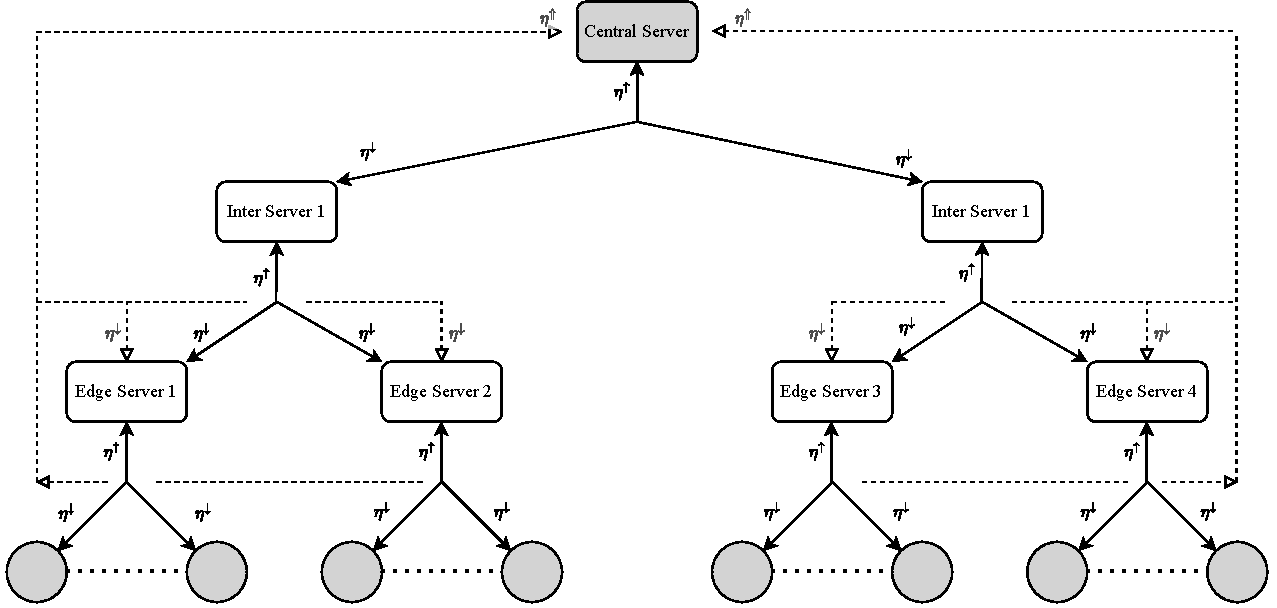
\includegraphics[clip,width=.8\columnwidth]{plots/Tree_Structure.drawio.pdf}
    \caption[System Diagram]{Diagramă a unui exemplu de sistem B-HFL. Liniile solide reprezintă legături de comunicare, în timp ce liniile punctate reprezintă conexiuni "reziduale" conceptuale, folosind legăturile de bază. Nodurile capabile de antrenament, cum ar fi clienții sau serverul central cu un set de date proxy, sunt în gri. Când parametrii modelului se propagă în sus, nodurile combină pseudo-gradienții de intrare și își actualizează modelul, folosind rata de învățare de la frunză către rădăcină $\eta^\uparrow$. La fel se întâmplă când parametrii curg de la nodurile părinte către nodurile copil cu rata de învățare $\eta^\downarrow$. Deoarece liniile punctate comunică de la $0$ la $K$ modele, $\eta^\Uparrow$ poate reprezenta de la $0$ la $K$ agregări, folosind o rată de învățare $\eta^\uparrow$.
    }\label{fig:TreeStructure}
\end{figure}

Un exemplu de sistem B-HFL, care ar fi principalul rezultat al acestei propuneri, poate fi văzut în \cref{fig:TreeStructure}. Serverul central controlează un set de date proxy folosit pentru antrenament post-agregare. Toate serverele își trimit actualizările către părinte după fiecare runda. Fiecare nod, inclusiv clienții, rulează cel puțin două optimizatoare FedOPT cu stări separate și rate de învățare, una pentru agregarea de la frunză către rădăcină cu pseudo-gradientul mediu $\Delta_t$ și una pentru agregarea părinților. Chiar dacă aceeași rată de învățare de la frunză la rădăcină $\eta^\uparrow$ și rata de învățare de la rădăcină la frunză $\eta^\downarrow$ ar fi utilizate pentru toate nodurile, stările independente ale optimizatorului serverului ar distinge procedura de agregare a nodului.

Conexiunile reziduale îndeplinesc funcții diferite între etapele de la frunză la rădăcină și de la rădăcină la frunză. Pentru etapa ascendentă, ele colectează actualizarea clientului cu valoarea absolută cea mai mare de la toate serverele edge, trimițând astfel un model suplimentar la serverul central pentru fiecare server edge. Serverul central poate apoi menține stări independente ale optimizatorului pentru fiecare conexiune "reziduală" de intrare. Pentru etapa descendentă, ele oferă serverelor edge șansa de a beneficia direct de antrenamentul serverului central fără a fi nevoie să se bazeze pe modelele diluate ale celor intermediare.



\section{Plan}
Familia de algoritmi prezentată pentru Învățarea Federată Ierarhică Bidirecțională va fi dezvoltată în perioada doctoratului și va face parte din teza finală de doctorat. În plus, înainte de teza finală, oferă oportunități pentru publicații la conferințe ce contribuie semnificativ la FL. Având în vedere noutatea FL în general și a HFL în particular, există un spațiu larg pentru dezvoltări ulterioare în structura B-HFL pe măsură ce domeniile se maturizează. Perioada de vară de la sfârșitul primului meu an de doctorat va fi dedicată implementării versiunii exemplu a B-HFL în cadrul framework-ului FL Flower~\citep{Flower} afiliat grupului nostru de cercetare. Acest framework este în prezent reglat pentru setările standard FL și ar necesita modificări importante ale API-ului pentru a executa și simula eficient HFL\@. Lucrările anterioare privind modelele la nivel de grup pentru Recunoașterea Activității Umane Federate ale \citet{OperaWorkshop} și motorul eficient de simulare FL la care am contribuit pot fi baza pentru implementarea sistemului.

Semestrul de toamnă, Michaelmas, al celui de-al doilea an va avea ca obiectiv principal publicarea unui articol de conferință bazat pe sistemul exemplu propus în Secțiunea \ref{sec:example_system}. Am discutat deja acest lucru cu supervizorul meu, Dr. Nicholas Lane, și am convenit că atât \href{https://iclr.cc/}{ICLR} cât și \href{https://mlsys.org/}{MLSys} ar fi conferințe potrivite. Având în vedere importanța crescândă a LLM-urilor și compromisurile recent descoperite de \citet{PersonalisationGeneralisationTradeoff} în ceea ce privește abilitățile lor de generalizare și personalizare, ele reprezintă o aplicație naturală pentru sistemul ierarhic propus. Mai mult, predicția textului în mai multe limbi oferă o aplicație FL, grupată în mod natural, corespunzătoare scenariilor din lumea reală în care țările au servere independente edge pentru FL și trebuie să colaboreze la un nivel continental și global. Studiul ar folosi un model BERT multilingv mare~\citep{RoBERTA} împreună cu două seturi de date multilingve~\citep[e.g., ][]{XGLUE,mC4} pentru antrenament. Un set de date va fi împărțit după limbă, iar celălalt va fi păstrat ca un set de date proxy la serverul central din \cref{fig:TreeStructure}. Obiectivele studiului ar fi să compare acuratețea finală a fiecărui model la fiecare nivel al ierarhiei pe seturile de test ale clienților și setul de test centralizat partiționat din setul de date proxy inițial. Așteptarea ar fi ca performanța modelului pe datele unui anumit client să fie proporțională cu proximitatea acestuia față de acel client în arbore. Alternativ, pentru setul de test proxy și uniunea tuturor seturilor de test ale clienților, acuratețea ar trebui să fie proporțională cu proximitatea față de serverul central. În plus, studii de ablație privind conexiunile "reziduale" sau optimizarea adaptivă vor fi efectuate. În cele din urmă, dacă timpul permite, lucrarea poate include alte sarcini grupate natural, cum ar fi recunoașterea vorbirii.

După publicarea acestei lucrări, o extensie naturală în semestrele Lent și Easter ar fi abordarea unui mediu în care clienții generează și șterg continuu date având memorie limitată. Sistemul exemplu ar fi extins pentru a permite antrenament asincron pe toate nodurile, inclusiv frunzele, care rulează în paralel cu componenta FL reală. Fiecare client ar genera un flux de date având o memorie internă fixă pe care să opereze în timpul antrenamentului. Constrângerile reale de resurse și asincronia pot fi modelate folosind clusterul Raspberry Pi FL de la Cambridge ML Systems. Această lucrare ar fi destinată pentru \href{https://sigmobile.org/mobicom/2023/}{MobiCom}, același loc unde am prezentat motorul de simulare Flower.

Dacă propunerea este reușită, cel de-al doilea an al doctoratului meu ar aduce o contribuție valoroasă în domeniul FL și s-ar concretiza în una sau mai multe publicații la conferințe împreuna cu o parte din teza finală. De asemenea, ar reprezenta o extensie majoră a framework-ului Flower~\citep{Flower} cu potențial pentru viitoare colaborări sau angajări în startup-ul \href{https://flower.dev/blog/2023-03-08-flower-labs/}{Flower Labs} finanțat de \href{https://www.ycombinator.com/}{Y Combinator}. După finalizarea doctoratului, intenționez să urmez o carieră în cercetarea privată sau academică.


% \clearpage
{\scriptsize
  \bibliography{thesis}}

\clearpage

%TC:ignore
\appendix
% \section{Appendix}
% \input{Files/appendix}
%TC:endignore
\end{document}